% Created by tikzDevice version 0.11 on 2018-04-09 15:27:54
% !TEX encoding = UTF-8 Unicode
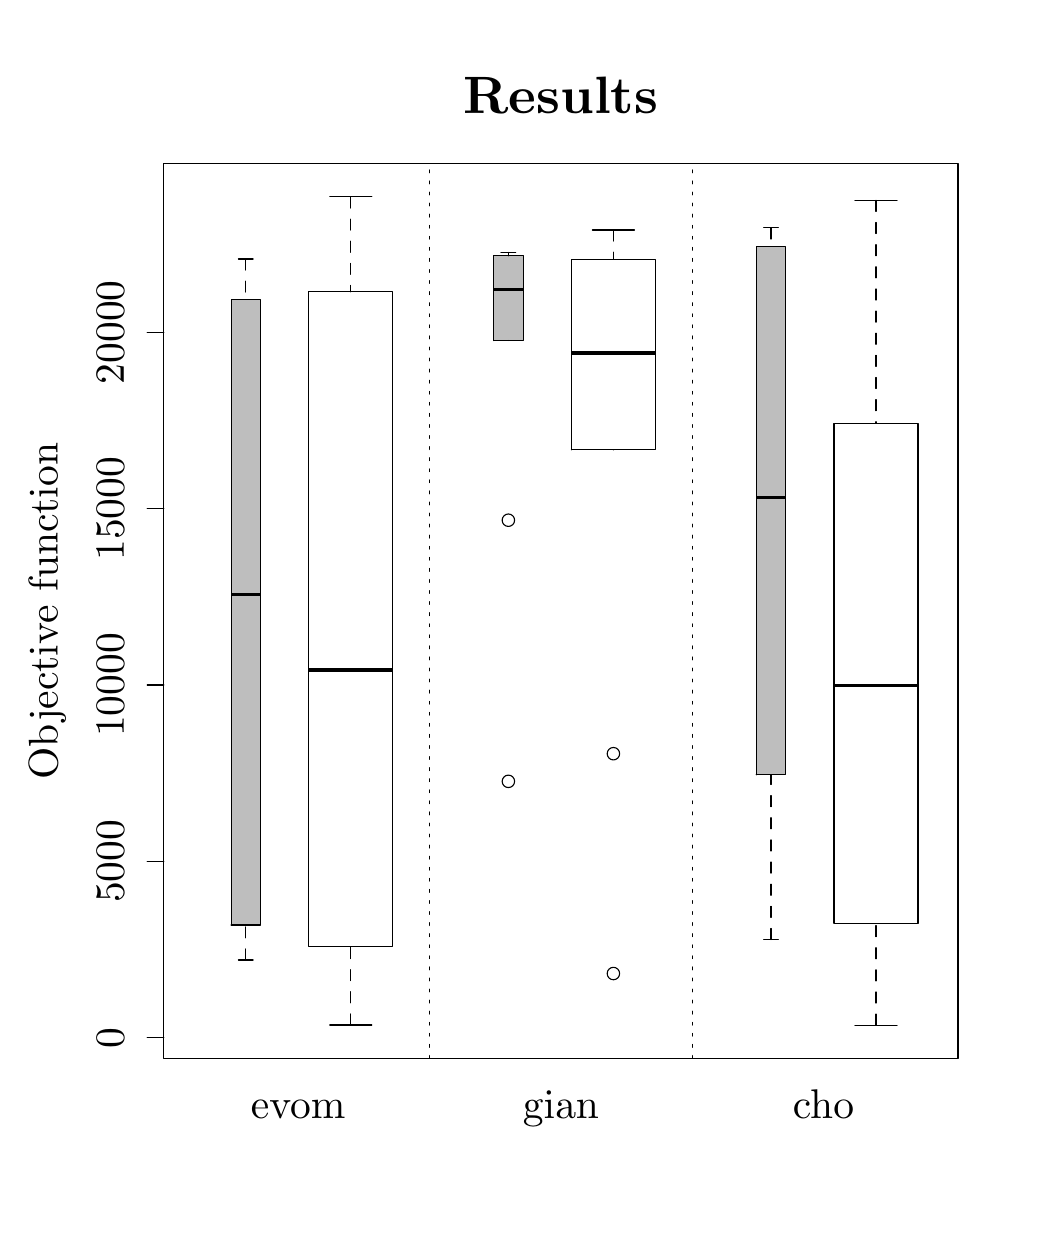
\begin{tikzpicture}[x=1pt,y=1pt]
\definecolor{fillColor}{RGB}{255,255,255}
\path[use as bounding box,fill=fillColor,fill opacity=0.00] (0,0) rectangle (361.35,433.62);
\begin{scope}
\path[clip] ( 49.20, 61.20) rectangle (336.15,384.42);
\definecolor{fillColor}{RGB}{190,190,190}

\path[fill=fillColor] ( 73.49,109.38) --
	( 84.12,109.38) --
	( 84.12,335.40) --
	( 73.49,335.40) --
	cycle;
\definecolor{drawColor}{RGB}{0,0,0}

\path[draw=drawColor,line width= 1.2pt,line join=round] ( 73.49,228.83) -- ( 84.12,228.83);

\path[draw=drawColor,line width= 0.4pt,dash pattern=on 4pt off 4pt ,line join=round,line cap=round] ( 78.81, 96.71) -- ( 78.81,109.38);

\path[draw=drawColor,line width= 0.4pt,dash pattern=on 4pt off 4pt ,line join=round,line cap=round] ( 78.81,350.04) -- ( 78.81,335.40);

\path[draw=drawColor,line width= 0.4pt,line join=round,line cap=round] ( 76.15, 96.71) -- ( 81.46, 96.71);

\path[draw=drawColor,line width= 0.4pt,line join=round,line cap=round] ( 76.15,350.04) -- ( 81.46,350.04);

\path[draw=drawColor,line width= 0.4pt,line join=round,line cap=round] ( 73.49,109.38) --
	( 84.12,109.38) --
	( 84.12,335.40) --
	( 73.49,335.40) --
	( 73.49,109.38);
\definecolor{fillColor}{RGB}{255,255,255}

\path[fill=fillColor] (101.58,101.70) --
	(131.94,101.70) --
	(131.94,338.19) --
	(101.58,338.19) --
	cycle;

\path[draw=drawColor,line width= 1.2pt,line join=round] (101.58,201.56) -- (131.94,201.56);

\path[draw=drawColor,line width= 0.4pt,dash pattern=on 4pt off 4pt ,line join=round,line cap=round] (116.76, 73.25) -- (116.76,101.70);

\path[draw=drawColor,line width= 0.4pt,dash pattern=on 4pt off 4pt ,line join=round,line cap=round] (116.76,372.45) -- (116.76,338.19);

\path[draw=drawColor,line width= 0.4pt,line join=round,line cap=round] (109.17, 73.25) -- (124.35, 73.25);

\path[draw=drawColor,line width= 0.4pt,line join=round,line cap=round] (109.17,372.45) -- (124.35,372.45);

\path[draw=drawColor,line width= 0.4pt,line join=round,line cap=round] (101.58,101.70) --
	(131.94,101.70) --
	(131.94,338.19) --
	(101.58,338.19) --
	(101.58,101.70);
\definecolor{fillColor}{RGB}{190,190,190}

\path[fill=fillColor] (168.38,320.56) --
	(179.01,320.56) --
	(179.01,351.13) --
	(168.38,351.13) --
	cycle;

\path[draw=drawColor,line width= 1.2pt,line join=round] (168.38,338.97) -- (179.01,338.97);

\path[draw=drawColor,line width= 0.4pt,dash pattern=on 4pt off 4pt ,line join=round,line cap=round] (173.70,320.56) -- (173.70,320.56);

\path[draw=drawColor,line width= 0.4pt,dash pattern=on 4pt off 4pt ,line join=round,line cap=round] (173.70,352.37) -- (173.70,351.13);

\path[draw=drawColor,line width= 0.4pt,line join=round,line cap=round] (171.04,320.56) -- (176.35,320.56);

\path[draw=drawColor,line width= 0.4pt,line join=round,line cap=round] (171.04,352.37) -- (176.35,352.37);

\path[draw=drawColor,line width= 0.4pt,line join=round,line cap=round] (168.38,320.56) --
	(179.01,320.56) --
	(179.01,351.13) --
	(168.38,351.13) --
	(168.38,320.56);

\path[draw=drawColor,line width= 0.4pt,line join=round,line cap=round] (173.70,255.64) circle (  2.25);

\path[draw=drawColor,line width= 0.4pt,line join=round,line cap=round] (173.70,161.28) circle (  2.25);
\definecolor{fillColor}{RGB}{255,255,255}

\path[fill=fillColor] (196.47,281.03) --
	(226.84,281.03) --
	(226.84,349.91) --
	(196.47,349.91) --
	cycle;

\path[draw=drawColor,line width= 1.2pt,line join=round] (196.47,316.10) -- (226.84,316.10);

\path[draw=drawColor,line width= 0.4pt,dash pattern=on 4pt off 4pt ,line join=round,line cap=round] (211.65,281.03) -- (211.65,281.03);

\path[draw=drawColor,line width= 0.4pt,dash pattern=on 4pt off 4pt ,line join=round,line cap=round] (211.65,360.49) -- (211.65,349.91);

\path[draw=drawColor,line width= 0.4pt,line join=round,line cap=round] (204.06,281.03) -- (219.24,281.03);

\path[draw=drawColor,line width= 0.4pt,line join=round,line cap=round] (204.06,360.49) -- (219.24,360.49);

\path[draw=drawColor,line width= 0.4pt,line join=round,line cap=round] (196.47,281.03) --
	(226.84,281.03) --
	(226.84,349.91) --
	(196.47,349.91) --
	(196.47,281.03);

\path[draw=drawColor,line width= 0.4pt,line join=round,line cap=round] (211.65, 91.83) circle (  2.25);

\path[draw=drawColor,line width= 0.4pt,line join=round,line cap=round] (211.65,171.27) circle (  2.25);
\definecolor{fillColor}{RGB}{190,190,190}

\path[fill=fillColor] (263.27,163.60) --
	(273.90,163.60) --
	(273.90,354.52) --
	(263.27,354.52) --
	cycle;

\path[draw=drawColor,line width= 1.2pt,line join=round] (263.27,263.84) -- (273.90,263.84);

\path[draw=drawColor,line width= 0.4pt,dash pattern=on 4pt off 4pt ,line join=round,line cap=round] (268.59,104.12) -- (268.59,163.60);

\path[draw=drawColor,line width= 0.4pt,dash pattern=on 4pt off 4pt ,line join=round,line cap=round] (268.59,361.25) -- (268.59,354.52);

\path[draw=drawColor,line width= 0.4pt,line join=round,line cap=round] (265.93,104.12) -- (271.24,104.12);

\path[draw=drawColor,line width= 0.4pt,line join=round,line cap=round] (265.93,361.25) -- (271.24,361.25);

\path[draw=drawColor,line width= 0.4pt,line join=round,line cap=round] (263.27,163.60) --
	(273.90,163.60) --
	(273.90,354.52) --
	(263.27,354.52) --
	(263.27,163.60);
\definecolor{fillColor}{RGB}{255,255,255}

\path[fill=fillColor] (291.36,110.06) --
	(321.73,110.06) --
	(321.73,290.69) --
	(291.36,290.69) --
	cycle;

\path[draw=drawColor,line width= 1.2pt,line join=round] (291.36,196.02) -- (321.73,196.02);

\path[draw=drawColor,line width= 0.4pt,dash pattern=on 4pt off 4pt ,line join=round,line cap=round] (306.54, 73.17) -- (306.54,110.06);

\path[draw=drawColor,line width= 0.4pt,dash pattern=on 4pt off 4pt ,line join=round,line cap=round] (306.54,371.21) -- (306.54,290.69);

\path[draw=drawColor,line width= 0.4pt,line join=round,line cap=round] (298.95, 73.17) -- (314.14, 73.17);

\path[draw=drawColor,line width= 0.4pt,line join=round,line cap=round] (298.95,371.21) -- (314.14,371.21);

\path[draw=drawColor,line width= 0.4pt,line join=round,line cap=round] (291.36,110.06) --
	(321.73,110.06) --
	(321.73,290.69) --
	(291.36,290.69) --
	(291.36,110.06);
\end{scope}
\begin{scope}
\path[clip] (  0.00,  0.00) rectangle (361.35,433.62);
\definecolor{drawColor}{RGB}{0,0,0}

\node[text=drawColor,rotate= 90.00,anchor=base,inner sep=0pt, outer sep=0pt, scale=  1.50] at ( 10.80,222.81) {Objective function};
\end{scope}
\begin{scope}
\path[clip] ( 49.20, 61.20) rectangle (336.15,384.42);
\definecolor{drawColor}{RGB}{0,0,0}

\path[draw=drawColor,line width= 0.4pt,dash pattern=on 1pt off 3pt ,line join=round,line cap=round] (145.23, 61.20) -- (145.23,384.42);

\path[draw=drawColor,line width= 0.4pt,dash pattern=on 1pt off 3pt ,line join=round,line cap=round] (240.12, 61.20) -- (240.12,384.42);
\end{scope}
\begin{scope}
\path[clip] (  0.00,  0.00) rectangle (361.35,433.62);
\definecolor{drawColor}{RGB}{0,0,0}

\node[text=drawColor,anchor=base,inner sep=0pt, outer sep=0pt, scale=  1.50] at ( 97.78, 39.60) {evom};

\node[text=drawColor,anchor=base,inner sep=0pt, outer sep=0pt, scale=  1.50] at (192.67, 39.60) {gian};

\node[text=drawColor,anchor=base,inner sep=0pt, outer sep=0pt, scale=  1.50] at (287.57, 39.60) {cho};
\end{scope}
\begin{scope}
\path[clip] (  0.00,  0.00) rectangle (361.35,433.62);
\definecolor{drawColor}{RGB}{0,0,0}

\node[text=drawColor,anchor=base,inner sep=0pt, outer sep=0pt, scale=  1.90] at (192.68,402.46) {\bfseries Results};
\end{scope}
\begin{scope}
\path[clip] (  0.00,  0.00) rectangle (361.35,433.62);
\definecolor{drawColor}{RGB}{0,0,0}

\path[draw=drawColor,line width= 0.4pt,line join=round,line cap=round] ( 49.20, 68.62) -- ( 49.20,323.53);

\path[draw=drawColor,line width= 0.4pt,line join=round,line cap=round] ( 49.20, 68.62) -- ( 43.20, 68.62);

\path[draw=drawColor,line width= 0.4pt,line join=round,line cap=round] ( 49.20,132.35) -- ( 43.20,132.35);

\path[draw=drawColor,line width= 0.4pt,line join=round,line cap=round] ( 49.20,196.08) -- ( 43.20,196.08);

\path[draw=drawColor,line width= 0.4pt,line join=round,line cap=round] ( 49.20,259.80) -- ( 43.20,259.80);

\path[draw=drawColor,line width= 0.4pt,line join=round,line cap=round] ( 49.20,323.53) -- ( 43.20,323.53);

\node[text=drawColor,rotate= 90.00,anchor=base,inner sep=0pt, outer sep=0pt, scale=  1.50] at ( 34.80, 68.62) {0};

\node[text=drawColor,rotate= 90.00,anchor=base,inner sep=0pt, outer sep=0pt, scale=  1.50] at ( 34.80,132.35) {5000};

\node[text=drawColor,rotate= 90.00,anchor=base,inner sep=0pt, outer sep=0pt, scale=  1.50] at ( 34.80,196.08) {10000};

\node[text=drawColor,rotate= 90.00,anchor=base,inner sep=0pt, outer sep=0pt, scale=  1.50] at ( 34.80,259.80) {15000};

\node[text=drawColor,rotate= 90.00,anchor=base,inner sep=0pt, outer sep=0pt, scale=  1.50] at ( 34.80,323.53) {20000};

\path[draw=drawColor,line width= 0.4pt,line join=round,line cap=round] ( 49.20, 61.20) --
	(336.15, 61.20) --
	(336.15,384.42) --
	( 49.20,384.42) --
	( 49.20, 61.20);
\end{scope}
\end{tikzpicture}
